\section{Proof of Theorem \ref{thm:g}}\label{sec: g}
Our proof of the Theorem~\ref{thm:g} relies on the following two inequalities for modular objects.
\begin{proposition}\label{prop:ineqA}\uses{lemma:ineqABnew-equiv, lemma:F-G-phi-psi-identities, lemma:F-G-pos, cor:ineqAnew}
Consider the function $A:(0,\infty)\to\C$ defined as
\begin{equation}\label{eqn:defA}
A(t):=-t^2\phi_0(i/t)-\frac{36}{\pi^2}\,\psi_I(it).
\end{equation}
Then
\begin{equation}\label{eqn:ineqA}
  A(t) < 0
\end{equation}
for all $t > 0$.
\end{proposition}

\begin{proposition}\label{prop:ineqB}\uses{lemma:ineqABnew-equiv, lemma:F-G-phi-psi-identities, cor:ineqBnew}
Consider the function $B:(0,\infty)\to\C$ defined as
\begin{equation}\label{eqn:defB}
  B(t) := -t^2\phi_0(i/t)+\frac{36}{\pi^2}\,\psi_I(it)
\end{equation}
Then
\begin{equation}\label{eqn:ineqB}
  B(t) > 0
\end{equation}
for all $t > 0$.
\end{proposition}

Here we formalize the proof of the inequalities by Lee \cite{Lee}.
First, we can rewrite the inequality in \ref{prop:ineqA} as follows.

\begin{definition}
Define two (quasi) modular forms as
\begin{align}
  F(z) &= (E_2(z) E_4(z) - E_6(z))^2 \label{eqn:defF} \\
  G(z) &= H_2(z)^{3} (2 H_{2}(z)^{2} + 5 H_{2}(z) H_{4}(z) + 5 H_{4}(z)^{2}). \label{eqn:defG}
\end{align}
\end{definition}

\begin{lemma}\label{lemma:F-G-phi-psi-identities}\uses{lemma: psi I psi T psi S explicit, lemma:lv1-lv2-identities, lemma:jacobi-identity}
We have
\begin{align}
  \phi_0 &= \frac{F}{\Delta} \label{eqn:phi0-F} \\
  \psi_S &= -\frac{1}{2} \frac{G}{\Delta}\label{eqn:psiS-G}
\end{align}
\end{lemma}
\begin{proof}
\eqref{eqn:phi0-F} is clear.
For \eqref{eqn:psiS-G}, using \eqref{eqn: psi S explicit} and \eqref{eqn:jacobi-identity} gives
\begin{align}
  \psi_S &= -128 \frac{H_3 + H_2}{H_4^2} - 128 \frac{H_2 - H_4}{H_3^2} \\
  &= -128 \frac{H_3^2 (H_2 - H_4) + H_4^2 (H_2 - H_4)}{H_3^2 H_4^2} \\
  &= -128 \frac{(H_2 + H_4)^2 (2H_2 + H_4) + H_4^2(H_2 + H_4)}{H_3^2 H_4^2} \\
  &= -128 \frac{H_2 (2H_2^2 + 5 H_2 H_4 + 5 H_4^2)}{H_3^2 H_4^2} \\
  &= -128 \frac{H_2^3 (2H_2^2 + 5 H_2 H_4 + 5 H_4^2)}{H_2^2 H_3^2 H_4^2} \\
  &= - \frac{1}{2} \frac{G}{\Delta}.
\end{align}
\end{proof}

\begin{lemma}\label{lemma:ineqABnew-equiv}\uses{lemma:F-G-phi-psi-identities, def: psi I psi T psi S, cor:disc-pos}
Inequality \eqref{eqn:ineqA} and \eqref{eqn:ineqB} are equivalent to
\begin{align}
  F(it) + \frac{18}{\pi^2} G(it) > 0 \label{eqn:ineqAnew} \\
  F(it) - \frac{18}{\pi^2} G(it) > 0 \label{eqn:ineqBnew}
\end{align}
respectively.
\end{lemma}
\begin{proof}
By \eqref{eqn: psi S define},
\begin{equation}
  \psi_I(it) = (\psi_S|_{-2}S)(it) = (it)^{2}\psi_S\left(-\frac{1}{it}\right) = -t^2 \psi_S\left(\frac{i}{t}\right).
\end{equation}
Combined with Lemma \ref{lemma:F-G-phi-psi-identities} we can rewrite \eqref{eqn:ineqA} as
\begin{equation}
  A(t) = -t^2 \phi_0\left(\frac{i}{t}\right) + \frac{36}{\pi^2} \psi_S\left(\frac{i}{t}\right) < 0 \Leftrightarrow \frac{F(it)}{\Delta(it)} + \frac{18}{\pi^2} \frac{G(it)}{\Delta(it)} > 0
\end{equation}
for $t > 0$, which is equivalent to \eqref{eqn:ineqAnew} by Corollary \ref{cor:disc-pos}.
Equivalences of \eqref{eqn:ineqB} and \eqref{eqn:ineqBnew} follows similarly; just change the sign.
\end{proof}


Now, the first inequality \eqref{eqn:ineqAnew} follows from the positivity of each $F(it)$ and $G(it)$.

\begin{lemma}\label{lemma:F-G-pos}\uses{thm:ramanujan-formula, lemma:theta-pos}
For all $t > 0$, we have $F(it) > 0$ and $G(it) > 0$.
\end{lemma}
\begin{proof}
By Ramanujan's identity \eqref{eqn:DE4}, we have $F(z) = 9 E_4'(z)^2$ and
\begin{equation}
  F(it) = 9E_4'(it)^2 = 9 \left(240\sum_{n \geq 1} n \sigma_3(n) e^{-2 \pi n t} \right) > 0.
\end{equation}
$G(it) > 0$ follows from positivity of $H_2(it)$ and $H_4(it)$ (Lemma \ref{lemma:theta-pos}).
\end{proof}

\begin{corollary}\label{cor:ineqAnew}\uses{lemma:F-G-pos}
\eqref{eqn:ineqAnew} holds.
\end{corollary}
\begin{proof}
This directly follows from Lemma \ref{lemma:F-G-pos}.
\end{proof}

To prove the second inequality \eqref{eqn:ineqBnew}, we need some identities satisfied by $F$ and $G$.
\begin{lemma}\label{lemma:F-G-de}\uses{thm:ramanujan-formula, thm:serre-der-prod-rule, prop:theta-der, lemma:lv1-lv2-identities}
$F$ and $G$ satisfy the following differential equations:
\begin{align}
    \partial_{12}\partial_{10} F - \frac{5}{6} E_{4} F &= 7200 \Delta (-E_{2}') \label{eqn:ddf} \\
    \partial_{12}\partial_{10} G - \frac{5}{6} E_{4} G &= -640 \Delta H_{2} \label{eqn:ddg}
\end{align}
\end{lemma}
\begin{proof}
Both can be shown by direct computations.
By Ramanujan's identities (Theorem \ref{thm:ramanujan-formula}) and the product rule of Serre derivatives (Theorem \ref{thm:serre-der-prod-rule}), we have
\begin{align}
  \partial_{5} (E_2 E_4 - E_6) &= (E_2 E_4 - E_6)' - \frac{5}{12} E_2 (E_2 E_4 - E_6) \\
  &= \frac{E_2^2 - E_4}{12} \cdot E_4 + E_2 \cdot \frac{E_2 E_4 - E_6}{3} - \frac{E_2 E_6 - E_4^2}{2} - \frac{5}{12}E_2 (E_2 E_4 - E_6) \\
  &= -\frac{5}{12} (E_2 E_6 - E_4^2) \label{eqn:S5} \\
  \partial_{7} (E_2 E_6 - E_4^2) &= (E_2 E_6 - E_4^2)' - \frac{7}{12} E_2 (E_2 E_6 - E_4^2) \\
  &= \frac{E_2^2 - E_4}{12} \cdot E_6 + E_2 \cdot \frac{E_2 E_6 - E_4^2}{2} - 2 E_4 \cdot \frac{E_2 E_4 - E_6}{3} - \frac{7}{12} E_2 (E_2 E_6 - E_4^2) \\
  &= -\frac{7}{12} E_4 (E_2 E_4 - E_6) \label{eqn:S7}
\end{align}
and using these we can compute
\begin{align}
  \partial_{10} F &= \partial_{10} (E_2 E_4 - E_6)^2 \\
  &= 2 (E_2 E_4 - E_6) \partial_{5} (E_2 E_4 - E_6) \\
  &= -\frac{6}{5} (E_2 E_4 - E_6) (E_2 E_6 - E_4^2), \\
  \partial_{12}\partial_{10} F &= -\frac{5}{6} \partial_{12} ((E_2 E_4 - E_6) (E_2 E_6 - E_4)) \\
  &= -\frac{5}{6} (\partial_{5}(E_2 E_4 - E_6)) (E_2 E_6 - E_4^2) - \frac{5}{6} (E_2 E_4 - E_6) (\partial_{7} (E_2 E_6 - E_4)) \\
  &= \frac{25}{72} (E_2 E_6 - E_4^2)^2 + \frac{35}{72} E_4 (E_2 E_4 - E_6)^2, \\
  \partial_{12}\partial_{10}F - \frac{5}{6} E_4 F &= \frac{25}{72}(E_2 E_6 - E_4^2)^2 + \frac{35}{72} E_4 (E_2 E_4 - E_6)^2 - \frac{5}{6} E_4 (E_2 E_4 - E_6)^2 \\
  &= \frac{25}{72} ((E_2 E_6 - E_4^2)^2 - E_4 (E_2 E_4 - E_6)^2) \\
  &= \frac{25}{72} (- E_2^2 E_4^3 + E_2^2 E_6^2 + E_4^4 - E_4 E_6^3) \\
  &= -\frac{25}{72} (E_4^3 - E_6^2) (E_2^2 - E_4) \\
  &= 7200 \cdot \frac{E_4^3 - E_6^2}{1728} \cdot \frac{-E_2^2 + E_4}{12}\\
  &= 7200 \Delta (-E_2')
\end{align}
which proves \eqref{eqn:ddf}.
Similarly, \eqref{eqn:ddg} can be proved using Proposition \ref{prop:theta-der} and Lemma \ref{lemma:lv1-lv2-identities}.
\end{proof}

\begin{corollary}\label{cor:F-G-de}\uses{lemma:F-G-de}
\eqref{eqn:ddf} (resp. \eqref{eqn:ddg}) is positive (resp. negative) on the (positive) imaginary axis.
\end{corollary}
\begin{proof}
\end{proof}


The second inequality \eqref{eqn:ineqBnew} follows from the following two observations.
Since $G(it) > 0$ for all $t > 0$, we can define the quotient
\begin{equation}\label{eqn:Q}
  Q(t) := \frac{F(it)}{G(it)}
\end{equation}
as a function on $(0, \infty)$.

\begin{lemma}\label{lemma:Qlim}\uses{lemma:E2-transform, lemma:Ek-is-modular-form, lemma:theta-transform-S-T}
We have
\begin{equation}\label{eqn:Qlim}
  \lim_{t \to 0^+} Q(t) = \frac{18}{\pi^2}.
\end{equation}
\end{lemma}
\begin{proof}
We have
\begin{equation}
  \lim_{t \to 0^+} Q(t) = \lim_{t \to 0^+} \frac{F(it)}{G(it)} = \lim_{t \to \infty} \frac{F(i/t)}{G(i/t)}.
\end{equation}
By using the transformation laws of Eisenstein series \eqref{eqn:E2-S-transform}, \eqref{eqn:Ek-trans-S} (for $k = 4, 6$) and the thetanull functions, \eqref{eqn:H2-transform-S}, \eqref{eqn:H4-transform-S}, we get
\begin{align}
    F\left(\frac{i}{t}\right) &= t^{12} F(it) - \frac{12t^{11}}{\pi} (E_2(it)E_4(it) - E_6(it))E_4(it) + \frac{36t^{10}}{\pi^2}E_4(it)^2, \\
    G\left(\frac{i}{t}\right) &= t^{10} H_{4}(it)^{3}(2H_{4}(it)^{2} + 5 H_{4}(it)H_{2}(it) + 5 H_{2}(it)^{2}).
\end{align}
Since $F$, $E_2 E_4 - E_6$ and $H_2$ are cusp forms, we have $\lim_{t \to \infty}t^k A(it) = 0$ when $A(z)$ is one of these forms and $k \geq 0$.
From $\lim_{t \to \infty} E_4(it) = 1 = \lim_{t \to \infty}H_{4}(it)$, we get
\begin{align}
    \lim_{t \to \infty} \frac{F(i/t)}{G(i/t)}
    &= \lim_{t \to \infty} \frac{t^{12} F(it) - \frac{12t^{11}}{\pi} (E_2(it)E_4(it) - E_6(it))E_4(it) + \frac{36t^{10}}{\pi^2}E_4(it)^2}{t^{10} H_{4}(it)^{3}(2H_{4}(it)^{2} + 5 H_{4}(it)H_{2}(it) + 5 H_{2}(it)^{2})} \\
    &= \lim_{t \to \infty} \frac{t^{2} F(it) - \frac{12t}{\pi} (E_2(it)E_4(it) - E_6(it))E_4(it) + \frac{36}{\pi^2}E_4(it)^2}{H_{4}(it)^{3}(2H_{4}(it)^{2} + 5 H_{4}(it)H_{2}(it) + 5 H_{2}(it)^{2})} \\
    &= \frac{18}{\pi^2}.
\end{align}
\end{proof}

\begin{proposition}\label{prop:Qdec}\uses{thm:ramanujan-formula, thm:serre-der-prod-rule, cor:F-G-de, thm:anti-serre-der-pos}
The function $t \mapsto Q(t)$ is monotone decreasing.
\end{proposition}

\begin{proof}
It is enough to show that
\begin{align}
    \frac{\dd}{\dd t} \left(\frac{F(it)}{G(it)}\right) < 0 &\Leftrightarrow (- 2\pi) \frac{F'(it)G(it) - F(it) G'(it)}{G(it)^{2}} < 0 \\
    &\Leftrightarrow F'(it) G(it) - F(it) G'(it) > 0 \\
    &\Leftrightarrow (\partial_{10}F)(it) G(it) - F(it) (\partial_{10}G)(it) > 0.
\end{align}
Let $\mathcal{L}_{1, 0} := (\partial_{10}F) G - F (\partial_{10} G)$.
Then its Fourier expansion starts with
\[
    \mathcal{L}_{1, 0} = 5308416000 q^{\frac{7}{2}} + O(q^{\frac{9}{2}})
\]
and its Serre derivative $\partial_{22} \mathcal{L}_{1, 0}$ is positive by Corollary \ref{cor:F-G-de}:
\begin{align}
    \partial_{22} \mathcal{L}_{1, 0} = (\partial_{12} \partial_{10} F) G - F (\partial_{12}\partial_{10} G)
    = \Delta (7200 (-E_{2}') G + 640 H_2 F) > 0.
\end{align}
Hence $\mathcal{L}_{1, 0}(it) > 0$ by Theorem \ref{thm:anti-serre-der-pos}, and the monotonicity follows.
\end{proof}


\begin{corollary}\label{cor:ineqBnew} \uses{lemma:Qlim, prop:Qdec, lemma:F-G-pos}
\eqref{eqn:ineqBnew} holds.
\end{corollary}
\begin{proof}
\begin{equation}
  \frac{F(it)}{G(it)} = Q(t) < \lim_{u \to 0^+} Q(u) = \frac{18}{\pi^2}
\end{equation}
and by Lemma \ref{lemma:F-G-pos}, \eqref{eqn:ineqBnew} follows.
\end{proof}

% \noindent \textbf{Remark:} \emph{We might formalize the  original proof from \cite{Via2017} or the proof of Dan Romik ``On Viazovska’s modular form inequalities'' \cite{Romik2023}. Below is the proof from \cite{Via2017}.}
% \begin{proof}
% Function $A(t)$ is plotted in Figure~\ref{fig: A}.
% \begin{figure}[h!]
% \caption{Plot of the functions $A(t)$, $A^{(2)}_0(t)=-\frac{368640}{\pi^2}\,t^2\,e^{-\pi /t}$, and $A^{(1)}_\infty(t)=-\frac{72}{\pi^2}\,e^{2\pi t}+\frac{8640}{\pi}t-\frac{23328}{\pi^2}$.\label{fig: A}}
%   \centering
% 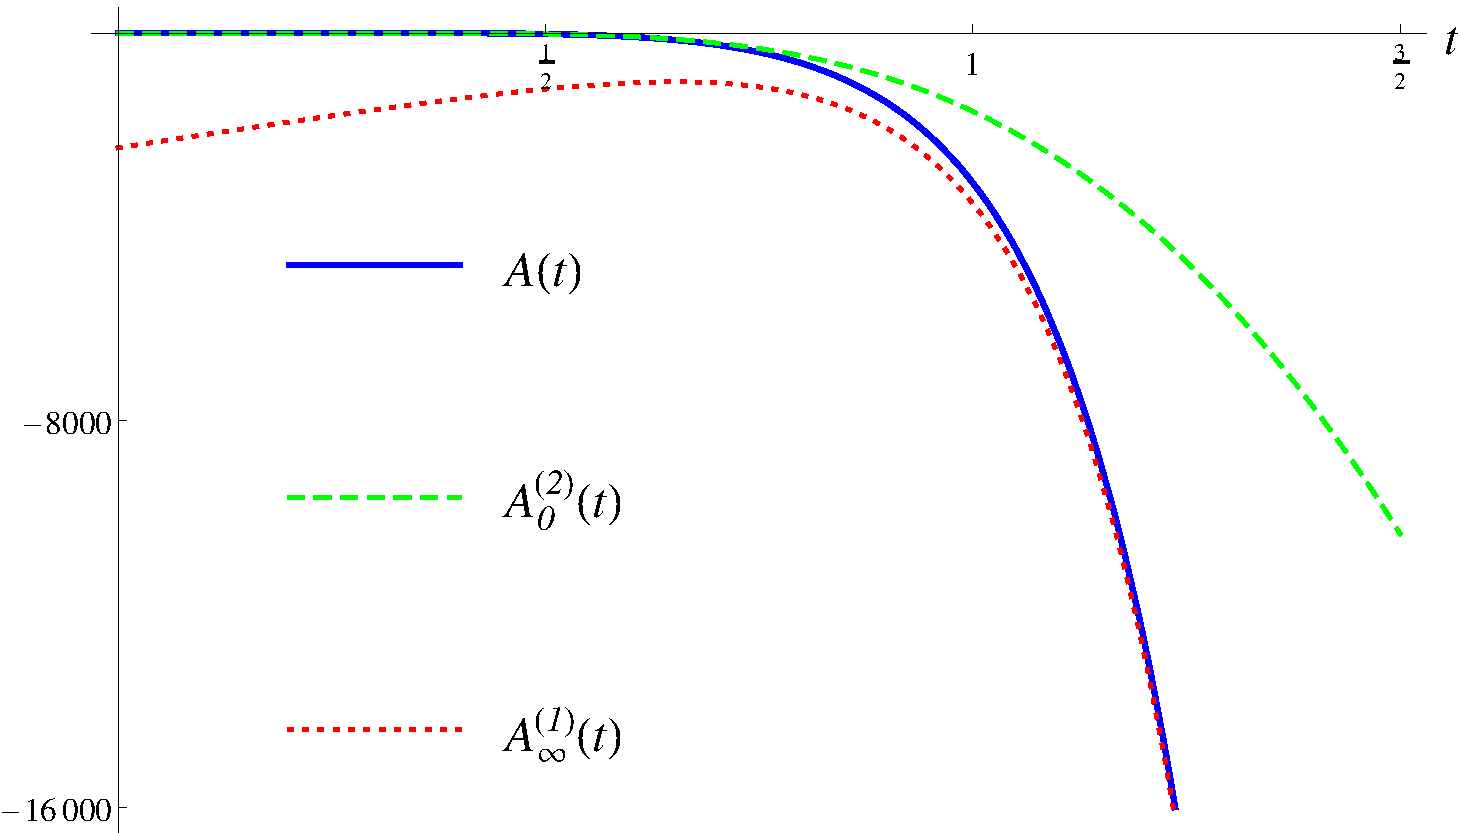
\includegraphics[width=300 pt]{graphics/e8plot_A.pdf}
% \end{figure}

% \noindent We observe that we can compute the values of $A(t)$ for $t\in(0,\infty)$ with any given precision. Indeed, from identities \eqref{eqn: phi0 transform} and \eqref{eqn: psi S define} we obtain the following two presentations for $A(t)$
% \begin{align}
%   A(t)=&-t^2\phi_0(i/t)+\frac{36}{\pi^2}\,t^2\,\psi_S(i/t)\notag\\
%   A(t)=&-t^2\phi_0(it)+\frac{12}{\pi}\,t\,\phi_{-2}(it)-\frac{36}{\pi^2}\,\phi_{-4}(it)-\frac{36}{\pi^2}\,\psi_I(i/t).\notag
% \end{align}
% For an integer $n\geq0$ let $A_0^{(n)}$ and  $A_{\infty}^{(n)}$ be the functions such that
% \begin{align}
%   A(t)=&A_0^{(n)}(t)+O(t^2\,e^{-\pi n /t})\quad\mbox{as}\;t\to0\label{eqn: A asymptotic expansion 0}\\
%   A(t)=&A_\infty^{(n)}(t)+O(t^2\,e^{-\pi n t})\quad\mbox{as}\;t\to\infty.\label{eqn: A asymptotic expansion infty}
% \end{align}
% For each $n\geq 0$ we can compute these functions from the Fourier expansions \eqref{eqn: phi fourier4}--\eqref{eqn: phi fourier0}, \eqref{eqn: psi fourier I}, and \eqref{eqn: psi fourier S}.
%   For example, from \eqref{eqn: phi fourier4}--\eqref{eqn: phi fourier0} and \eqref{eqn: psi fourier I} we compute
% %$$A_\infty^{(0)}(t)=-\frac{72}{\pi^2}\,e^{2\pi t}$$ and
% \begin{align}A_\infty^{(6)}(t)=&\scriptstyle-\tfrac{72}{\pi ^2}\, e^{2 \pi  t}-\tfrac{23328}{\pi ^2}+\tfrac{184320}{\pi ^2}\, e^{-\pi  t}-\tfrac{5194368}{\pi ^2}\, e^{-2 \pi  t}+\tfrac{22560768}{\pi ^2}\, e^{-3 \pi  t}-\tfrac{250583040}{\pi
%     ^2}\, e^{-4 \pi  t}+\tfrac{869916672 }{\pi ^2}\,e^{-5 \pi  t}\notag\\&\scriptstyle+t(\tfrac{8640}{\pi }+\tfrac{2436480}{\pi }\, e^{-2 \pi  t}+\tfrac{113011200 }{\pi }\,e^{-4 \pi  t})-t^2(518400\,e^{-2 \pi  t}+31104000\,e^{-4 \pi  t}).\notag
% \end{align}
% From \eqref{eqn: phi fourier4}--\eqref{eqn: phi fourier0} and \eqref{eqn: psi fourier S} we compute
% %$$A_0^{(2)}(t)=-\frac{368640}{\pi^2}\,t^2\,e^{-\pi /t}$$and
% $$A_0^{(6)}(t)=t^2(-\tfrac{368640}{\pi ^2}\, e^{-\pi/t}-518400\, e^{-2\pi/t}-\tfrac{45121536}{\pi ^2}\, e^{-3\pi/t}-31104000\,e^{-4\pi/t}-\tfrac{1739833344}{\pi ^2}\, e^{-5\pi/t}).$$
% Moreover, from the convergent asymptotic expansion for the Fourier coefficients of a weakly holomorphic modular form \cite[Proposition 1.12]{Bruinier} we find that the $n$-th Fourier coefficient $c_{\psi_I}(n)$ of $\psi_I$ satisfies
% \begin{equation}\label{eqn: Fourier estimate 1}|c_{\psi_I}(n)|\leq e^{4\pi\sqrt{n}}\qquad n\in\tfrac 12 \Z_{>0}.\end{equation} Similar inequalities hold for the Fourier coefficients of $\psi_S$, $\phi_0$, $\phi_{-2}$, and $\phi_{-4}$:
% \begin{align}\label{eqn: Fourier estimate 2}
% &|c_{\psi_S}(n)|\leq 2e^{4\pi\sqrt{n}}\qquad n\in\tfrac 12 \Z_{>0} \\
% &|c_{\phi_0}(n)|\leq 2e^{4\pi\sqrt{n}}\qquad n\in \Z_{>0} \\
% &|c_{\phi_{-2}}(n)|\leq e^{4\pi\sqrt{n}}\qquad n\in  \Z_{>0} \\
% &|c_{\phi_{-4}}(n)|\leq e^{4\pi\sqrt{n}}\qquad n\in \Z_{>0}. \label{eqn: Fourier estimate 5}
%   \end{align}
% Therefore, we can estimate the error terms in the asymptotic expansions \eqref{eqn: A asymptotic expansion 0} and \eqref{eqn: A asymptotic expansion infty} of $A(t)$
% \begin{align}
% \left|A(t)-A_0^{(m)}(t)\right|\leq& (t^2+\frac{36}{\pi^2})\,\sum_{n=m}^\infty 2e^{2\sqrt{2}\pi\sqrt{n}}\,e^{-\pi n/t}\notag\\
% \left|A(t)-A_\infty^{(m)}(t)\right|\leq& (t^2+\frac{12}{\pi}\,t+\frac{36}{\pi^2})\,\sum_{n=m}^\infty 2e^{2\sqrt{2}\pi\sqrt{n}}\,e^{-\pi nt}.\notag
% \end{align}
% For an integer $m\geq0$ we set
% \begin{align}
% R^{(m)}_0:=&(t^2+\frac{36}{\pi^2})\,\sum_{n=m}^\infty 2e^{2\sqrt{2}\pi\sqrt{n}}\,e^{-\pi n/t}\notag\\
% R^{(m)}_\infty:=&(t^2+\frac{12}{\pi}\,t+\frac{36}{\pi^2})\,\sum_{n=m}^\infty 2e^{2\sqrt{2}\pi\sqrt{n}}\,e^{-\pi nt}.\notag
% \end{align}
% Using interval arithmetic we check that
% \begin{align}
% &\left|R_0^{(6)}(t)\right|\leq\left|A_0^{(6)}(t)\right|\quad\mbox{ for }\;t\in(0,1]\notag\\
% &\left|R_\infty^{(6)}(t)\right|\leq\left|A_\infty^{(6)}(t)\right|\quad\mbox{ for }\;t\in[1,\infty)\notag\\
% &A_0^{(6)}(t)<0\quad\mbox{ for }\;t\in(0,1]\notag\\
% &A_\infty^{(6)}(t)<0\quad\mbox{ for }\;t\in[1,\infty).\notag
% \end{align}
% Thus, we see that $A(t)<0$ for $t\in (0,\infty)$. This finishes the proof of the Proposition.
% \end{proof}


% \noindent\textbf{Remark} \emph{Below is the proof from \cite{Via2017}. Similarly to the previous proposition, another (hopefully easier for the formalization) proof of this inequality is given in \cite{Romik2023}}.
% \begin{proof}

% The function $B$ can be also written as
% \begin{align}
%   B(t)=&-t^2\phi_0(i/t)-\frac{36}{\pi^2}\,t^2\,\psi_S(i/t)\notag\\
%   B(t)=&-t^2\phi_0(it)+\frac{12}{\pi}\,t\,\phi_{-2}(it)-\frac{36}{\pi^2}\,\phi_{-4}(it)+\frac{36}{\pi^2}\,\psi_I(i/t).\notag
% \end{align}
% Our aim is to prove that $B(t)>0$ for $t\in(0,\infty)$. A plot of $B(t)$ is given in Figure~\ref{fig:B}.
% \begin{figure}[h!]
% \caption{Plot of the functions $B(t)$, $B^{(2)}_0(t)=\frac{368640}{\pi^2}\,t^2\,e^{-\pi /t}$, and $B^{(1)}_\infty(t)=\frac{8640}{\pi}t-\frac{23328}{\pi^2}$.\label{fig:B}}
%   \centering
% 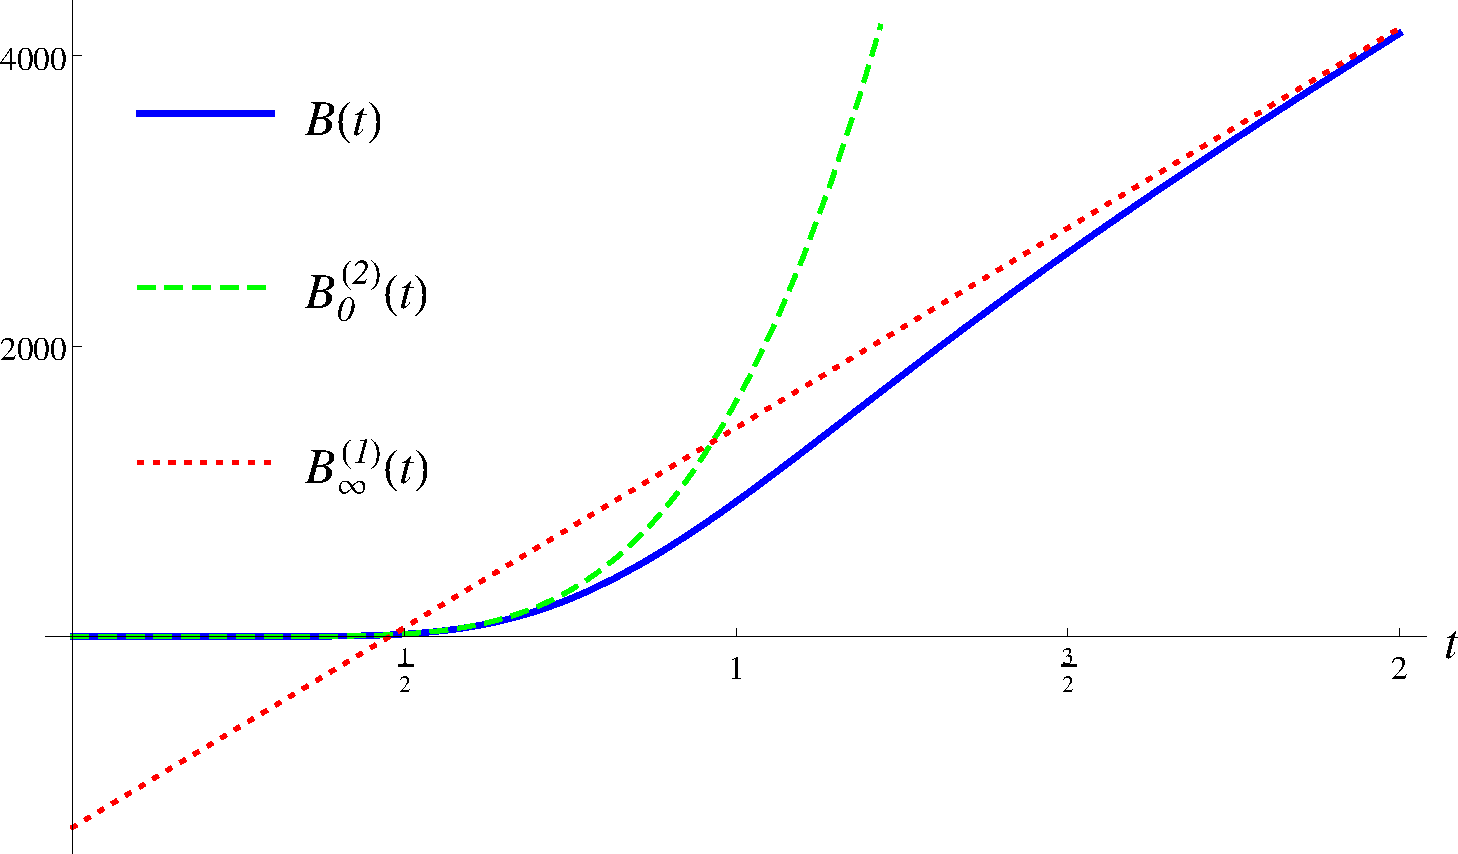
\includegraphics[width=300 pt]{graphics/e8plot_B.pdf}
% \end{figure}

% \noindent For $n\geq 0$ let $B_0^{(n)}$ and  $B_{\infty}^{(n)}$ be the functions  such that
% \begin{align}
%   B(t)=&B_0^{(n)}(t)+O(t^2\,e^{-\pi n /t})\quad\mbox{as}\;t\to0\notag\\
%   B(t)=&B_\infty^{(n)}(t)+O(t^2\,e^{-\pi n t})\quad\mbox{as}\;t\to\infty.\notag
% \end{align}
% We find
% \begin{align}B_\infty^{(6)}(t)=&-\tfrac{12960}{\pi ^2}-\tfrac{184320}{\pi ^2}\,\scriptstyle e^{-\pi  t}\displaystyle-\tfrac{116640}{\pi ^2} \,\scriptstyle e^{-2\pi  t}\displaystyle-\tfrac{22560768}{\pi ^2}\,\scriptstyle e^{-3\pi  t}\displaystyle+\tfrac{56540160}{\pi ^2}\,\scriptstyle e^{-4\pi  t}\displaystyle-\tfrac{869916672 }{\pi ^2} \,\scriptstyle e^{-5\pi  t}\displaystyle\notag\\
% &+t(\tfrac{8640 }{\pi }+\tfrac{2436480}{\pi }\,\scriptstyle e^{-2\pi  t}\displaystyle+\tfrac{113011200 }{\pi }\,\scriptstyle e^{-4\pi  t}\textstyle)-t^2(\scriptstyle518400\,\scriptstyle e^{-2\pi  t}\displaystyle+\scriptstyle31104000\,\scriptstyle e^{-4\pi  t}\displaystyle)\notag
% \end{align}
% and
% $$B_0^{(6)}(t)= t^2(\tfrac{368640}{\pi ^2}\, e^{-\pi/t}-518400\, e^{-2 \pi /t}+\tfrac{45121536 }{\pi ^2}\,e^{-3 \pi/t}-31104000\, e^{-4 \pi/t}+\tfrac{1739833344 }{\pi ^2}\,e^{-5 \pi/t}) .$$
% The estimates \eqref{eqn: Fourier estimate 1}--\eqref{eqn: Fourier estimate 5} imply that $$\left|B(t)-B_0^{(6)}(t)\right|\leq R_0^{(6)}(t)\quad\mbox{for}\;t\in(0,1]$$
% and
% $$\left|B(t)-B_\infty^{(6)}(t)\right|\leq R_\infty^{(6)}(t)\quad\mbox{for}\;t\in[1,\infty).$$
% Using interval arithmetic we verify that
% \begin{align}
% &\left|R_0^{(6)}(t)\right|\leq\left|B_0^{(6)}(t)\right|\quad\mbox{ for }\;t\in(0,1]\notag \\
% &\left|R_\infty^{(6)}(t)\right|\leq\left|B_\infty^{(6)}(t)\right|\quad\mbox{ for }\;t\in[1,\infty)\notag \\
% &B_0^{(6)}(t)>0\quad\mbox{ for }\;t\in(0,1]\notag \\
% &B_\infty^{(6)}(t)>0\quad\mbox{ for }\;t\in[1,\infty). \notag
% \end{align}
% Now identity \eqref{eqn:g B} implies \eqref{eqn:g2}.
% \end{proof}
Finally, we are ready to prove Theorem~\ref{thm:g}.
\begin{theorem}\label{thm:g1}
\uses{prop: a(r) double zeroes, prop: b(r) double zeroes, prop:ineqA, prop:ineqB}
The function
$$g(x):=\frac{\pi\,i}{8640}a(x)+\frac{i}{240\pi}\,b(x)$$
satisfies conditions \eqref{eqn:g1}--\eqref{eqn:g3}.
\end{theorem}
\begin{proof}
First, we prove that \eqref{eqn:g1} holds. By Propositions~\ref{prop: a(r) double zeroes} and \ref{prop: b(r) double zeroes} we know that for $r>\sqrt{2}$
\begin{equation}\label{eqn:g A} g(r)=\frac{\pi}{2160}\,\sin(\pi r^2/2)^2\,\int\limits_0^\infty A(t)\,e^{-\pi r^2 t}\,dt\end{equation}
where $$A(t)=-t^2\phi_0(i/t)-\frac{36}{\pi^2}\,\psi_I(it).$$
from the Proposition~\ref{prop:ineqA} we know that $A(t)<0\quad\mbox{for}\;t\in(0,\infty).$
Therefore identity \eqref{eqn:g A} implies \eqref{eqn:g1}.

Next, we prove \eqref{eqn:g2}. By Propositions~\ref{prop: a another integral} and~\ref{prop: b another integral} we know that for $r>0$
\begin{equation}\label{eqn:g B} \widehat{g}(r)=\frac{\pi}{2160}\,\sin(\pi r^2/2)^2\,\int\limits_0^\infty B(t)\,e^{-\pi r^2 t}\,dt\end{equation}
where $$B(t)=-t^2\phi_0(i/t)+\frac{36}{\pi^2}\,\psi_I(it).$$


Finally, the property \eqref{eqn:g3} readily follows from Proposition~\ref{prop: a values} and Proposition~\ref{prop: b values}.
This finishes the proof of Theorems~\ref{thm:g1} and~\ref{thm:g}.
\end{proof}
